% mnras_guide.tex
%
% MNRAS LaTeX user guide
%
% v3.1 released 11 June 2020
%
% v3.0 released 22 May 2015
% (version numbers match those of mnras.cls)
%
% Copyright (C) Royal Astronomical Society 2015
% Authors:
% Keith T. Smith (Royal Astronomical Society)

% Change log
%
% v3.0   September 2013 - May 2015
%    First version: complete rewrite of the user guide
%    Basic structure taken from mnras_template.tex by the same author

%%%%%%%%%%%%%%%%%%%%%%%%%%%%%%%%%%%%%%%%%%%%%%%%%%
% Basic setup. Most papers should leave these options alone.
\documentclass[fleqn,usenatbib,useAMS]{mnras}

%%%%% AUTHORS - PLACE YOUR OWN PACKAGES HERE %%%%%

% Only include extra packages if you really need them. Common packages are:
\usepackage{graphicx}	% Including figure files
\usepackage{amsmath}	% Advanced maths commands
\usepackage{amssymb}	% Extra maths symbols
\usepackage{multicol}        % Multi-column entries in tables
\usepackage{bm}		% Bold maths symbols, including upright Greek
\usepackage{pdflscape}	% Landscape pages

%%%%%%%%%%%%%%%%%%%%%%%%%%%%%%%%%%%%%%%%%%%%%%%%%%

%%%%%% AUTHORS - PLACE YOUR OWN MACROS HERE %%%%%%
\usepackage{subcaption}
% Please keep new commands to a minimum, and use \newcommand not \def to avoid
% overwriting existing commands. Example:
%\newcommand{\pcm}{\,cm$^{-2}$}	% per cm-squared
\newcommand{\kms}{\,km\,s$^{-1}$} % kilometres per second
\newcommand{\bibtex}{\textsc{Bib}\!\TeX} % bibtex. Not quite the correct typesetting, but close enough

%%%%%%%%%%%%%%%%%%%%%%%%%%%%%%%%%%%%%%%%%%%%%%%%%%
\usepackage{booktabs}
\usepackage{multirow}


\usepackage[section]{placeins} %ensures figures go in their section e.g https://tex.stackexchange.com/questions/279/how-do-i-ensure-that-figures-appear-in-the-section-theyre-associated-with

% Use vector fonts, so it zooms properly in on-screen viewing software
% Don't change these lines unless you know what you are doing
\usepackage[T1]{fontenc}
\usepackage{ae,aecompl}

% MNRAS is set in Times font. If you don't have this installed (most LaTeX
% installations will be fine) or prefer the old Computer Modern fonts, comment
% out the following line
\usepackage{newtxtext,newtxmath}
% Depending on your LaTeX fonts installation, you might get better results with one of these:
%\usepackage{mathptmx}
%\usepackage{txfonts}

%%%%%%%%%%%%%%%%%%% TITLE PAGE %%%%%%%%%%%%%%%%%%%

% Title of the paper, and the short title which is used in the headers.
% Keep the title short and informative.
	\title[Stochastic Kalman PTA]{State-space analysis of a continuous gravitational wave source with apulsar timing array: inclusion of the pulsar terms}

% The list of authors, and the short list which is used in the headers.
% If you need two or more lines of authors, add an extra line using \newauthor
\author[Kimpson]{Kimpson$^{1}$, O'Neil$^{2}$, Melatos$^{2}$, O'Leary, Evans$^{3}$, Moran, others, etc. etc.%
\thanks{Contact e-mail: \href{tom.kimpson@unimelb.edu.au}{tom.kimpson@unimelb.edu.au}}%
%\thanks{Present address: Science magazine, AAAS Science International, \mbox{82-88}~Hills Road, Cambridge CB2~1LQ, UK}%
\\
% List of institutions
$^{1}$School of Physics, University of Melbourne, Parkville, VIC 3010, Australia \\
$^{2}$OzGrav, University of Melbourne, Parkville, VIC 3010, Australia \\
$^{3}$Department of Electrical and Electronic Engineering, University of Melbourne, Parkville, Victoria 3010, Australia }

% These dates will be filled out by the publisher
%\date{Last updated 2020 June 10; in original form 2013 September 5}
\date{Last updated \today}

% Enter the current year, for the copyright statements etc.
\pubyear{2023}

% Don't change these lines
\begin{document}
\label{firstpage}
\pagerange{\pageref{firstpage}--\pageref{lastpage}}
\maketitle

% Abstract of the paper
\begin{abstract}	
\begin{itemize}
	\item PTAs can detect the nano-Hz GWs 
	\item The detection procedure can be formulated as a state-space method
	\item Previous state-space methods use frequencies
	\item We lift this limitation
\end{itemize}
\end{abstract}

% Select between one and six entries from the list of approved keywords.
% Don't make up new ones.
\begin{keywords}
gravitational waves -- methods: data analysis -- pulsars: general
\end{keywords}

%%%%%%%%%%%%%%%%%%%%%%%%%%%%%%%%%%%%%%%%%%%%%%%%%%

%%%%%%%%%%%%%%%%% BODY OF PAPER %%%%%%%%%%%%%%%%%%

% The MNRAS class isn't designed to include a table of contents, but for this document one is useful.
% I therefore have to do some kludging to make it work without masses of blank space.
\begingroup
\let\clearpage\relax
%\tableofcontents
\endgroup
\newpage




\section{Introduction}\label{sec:intro}

State-space methods have been shown \citep{KimpsonPTA1,KimpsonPTA2} to be a promising and complementary alternative to standard data analysis techniques for the detection of nanohertz gravitational waves (GWs) by pulsar timing arrays  \citep[PTAs;][]{Tiburzi2018, 2021hgwa.bookE...4V}. State-space methods self-consistently track the intrinsic timing noise in PTA pulsars \citep[e.g.][]{Shannon2010,Lasky2015,Caballero2016,Goncharov2021}, enabling the specific time-ordered realisation of the timing noise to be disentangled statistically from the GW-induced modulations. Conversely, traditional PTA analysis techniques average over the ensemble of possible timing noise realizations to obtain the noise power spectral density (PSD), and discards time-ordered information when taking the modulus of the complex Fourier phase in each PSD frequency bin. State-space methods are then complementary to traditional PTA analysis techniques for two reasons: (i) they track the actual noise realization rather than an ensemble average; (ii) they preserve time ordering by implicitly preserving the Fourier phases, which the PSD discards. State-space methods follow the customary signal processing approach in many industrial and scientific electrical engineering applications. \textcolor{red}{TK:CITATIONS HERE} \newline 


For the purposes of simplicity, and in order to maintain consistency with prior works applying state-space methods within neutron star astrophysics \citep[e.g.][]{Myers2021MNRAS.502.3113M,Meyers2021}, previous state-space PTA analysis techniques have accepted as an input a sequence of pulse frequencies. However, in order to analyse real data and make contact with traditional PTA analysis techniques it is necessary for state-space methods to accepted as an input traditional pulsar observables such as the pulsar phase or pulse time of arrival (ToA). \newline 


In this paper we take a step towards lifting the above limitation. We demonstrate how to extend previous PTA state-space methods to accept as an input the measured pulse phase. We show how the intrinsic pulse phase and the intrinsic frequency for each constituent pulsar in the PTA can be tracked using a Kalman filter \citep{Kalman1}. We combine the Kalman tracking of the intrinsic pulsar's states with a Bayesian nested samplers \citep{Skilling} to estimate the static parameters of a continuous, quasi-monochromatic GW source, and calculate the marginalized likelihood for model selection.




The paper is organised as follows. In Section \ref{sec:state_space_formulation} we... Throughout the paper we adopt natural units, with $c = G = \hbar =1 $












\section{State-space formulation}\label{sec:state_space_formulation}
In this section we formulate PTA detection of the stochastic GW background as a state-space problem. There are $N$ pulsars in the array, labelled $1\leq n\leq N$.  The $n$-th pulsar’s spin frequency $f_{\rm p}^{(n)}(t)$, as measured in the local, freely-falling rest frame of the pulsar’s centre of mass, evolves according to a stochastic differential equation. We adopt the phenomenological model for $f_{\rm p}^{(n)}(t)$ as a mean-reverting Ornstein-Uhlenbeck process also used in previous state-space analyses \citep{Vargas, KimpsonPTA1, KimpsonPTA2}. The $n$-th pulsar’s phase $\phi_{\rm p}^{(n)}(t)$ is the time integral of $f_{\rm p}^{(n)}(t)$. Section \ref{sec:spin_evolution} presents the dynamical equations for the evolution of the intrinsic states, $f_{\rm p}^{(n)}(t)$ and $\phi_{\rm p}^{(n)}(t)$. An observer at Earth measures the pulse phase  $\phi_{\rm m}^{(n)}(t)$. The relation between the states $f_{\rm p}^{(n)}(t)$, $\phi_{\rm p}^{(n)}(t)$ and the measurement, $\phi_{\rm m}^{(n)}(t)$, is described by a measurement equation which quantifies the influence of a continuous GW source and PTA instrumental noise. The model of the measurement equation is presented in Section \ref{sec:gw_background_modulation}. In Section \ref{sec:summary_of_static_parameters} we summarise the static parameters of the model. 





\subsection{Dynamical state evolution}\label{sec:spin_evolution}

The instantaneous phase of the $n$-th pulsar is the time integral of the rest frame spin frequency, which itself evolves according to a mean-reverting Ornstein-Uhlenbeck process, described by a Langevin equation with a time-dependent drift term \citep{Vargas}, viz.
\begin{align}
	\frac{d \phi_{\rm p}^{(n)}}{dt} &= f_{\rm p}^{(n)} \\ 
	\frac{df_{\rm p}^{(n)}}{dt} &= -\gamma^{(n)}	 [f_{\rm p}^{(n)} - f_{\rm em}^{(n)} (t)] + \dot{f}_{\rm em}^{(n)}(t) +\xi^{(n)}(t) \ , 
	\label{eq:frequency_evolution}
\end{align}
where $f_{\rm em}^{(n)}$ is the deterministic evolution, an overdot denotes a derivative with respect to $t$, $\gamma^{(n)}$ is a damping constant whose reciprocal specifies the mean-reversion timescale, and $\xi^{(n)}(t)$ is a white noise stochastic process which satisfies
\begin{align}
	\langle \xi^{(n)}(t) \rangle &= 0 \ , \\
	\langle \xi^{(n)}(t) \xi^{(n')}(t') \rangle &= [\sigma^{(n)}]^2 \delta_{n,n'} \delta(t - t') \ .	\label{eq:xieqn}
\end{align}
In Equation \eqref{eq:xieqn}, $[\sigma^{(n)}]^2$ parametrizes the noise amplitude and produces characteristic root mean square fluctuations $\approx \sigma^{(n)} / [\gamma^{(n)}]^{1/2}$ in $f_{\rm p}^{(n)}(t)$ \citep{gardiner2009stochastic}. The deterministic evolution $f_{\rm em}^{(n)}$ is attributed to magnetic dipole braking for the sake of definiteness, with braking index $n_{\rm em}=3$ \citep{1969ApJ...157..869G}. PTAs are typically composed of millisecond pulsars (MSPs), for which the quadratic correction due to $n_{\rm em}$ in $f_{\rm p}^{(n)}(t)$ is negligible over the observation time $T_{\rm obs} \sim 10 \, {\rm yr}$. Consequently, 	$f_{\rm em}^{(n)}(t)$ can be approximated accurately by 
\begin{equation}
	f_{\rm em}^{(n)}(t) = f_{\rm em}^{(n)}(t_1) + \dot{f}_{\rm em}^{(n)}(t_1)t \ , \label{eq:spinevol}
\end{equation} 
where $t_1$ labels the time of the first TOA. \newline 


\subsection{Modulation of the pulsar states by a GW}\label{sec:gw_background_modulation}
In the presence of a GW, $\phi_{\rm p}^{(n)}(t)$ is related to  $\phi_{\rm m}^{(n)}(t)$ and $f_{\rm m}^{(n)}(t)$ via a measurement equation,
\begin{equation}
	\phi_{\rm m}^{(n)}(t) = \phi_{\rm m}^{(n)}\left[t-d^{(n)}\right] - f_{\rm p}^{(n)}\left [t-d^{(n)} \right ] g^{(n)}(t) +  \varepsilon^{(n)}(t)\ ,
	\label{eq:measurement}
\end{equation}
where $d^{(n)}$ labels the distance to the $n$-th pulsar,  $\phi_{\rm m}^{(n)}$,$f_{\rm p}^{(n)}$ are evaluated at the retarded time $t-d^{(n)}$, and $\varepsilon^{(n)}(t)$ is a Gaussian measurement noise which satisfies 
\begin{align}
	\langle \varepsilon^{(n)}(t) \rangle &= 0 \ , \\
	\langle \varepsilon^{(n)}(t) \varepsilon^{(n')}(t') \rangle &= \sigma_{\rm m}^2 \delta_{n,n'} \delta(t - t') \ .	\label{eq:vareps}
\end{align}
In Equation \eqref{eq:vareps}, $\sigma_{\rm m}^2$ is the variance of the measurement noise at the telescope and is shared between all pulsars. In Equation \eqref{eq:measurement} the measurement function $g^{(n)}(t)$ is,
\begin{align}
	g^{(n)}(t) =& - \frac{ H_{ij}[q^{(n)}]^i [q^{(n)}]^j }{2 \Omega [1 + \boldsymbol{n}\cdot \boldsymbol{q}^{(n)}] } \nonumber \\
	& \times \Big[\sin\left(-\Omega t +\Phi_0\right) - \sin \left \{-\Omega t +\Phi_0 + \chi^{(n)} \right \} \Big ] \ ,
	\label{eq:g_func_trig}
\end{align}
where $[q^{(n)}]^i$ labels the $i$-th coordinate component of the $n$-th pulsar's position vector $\boldsymbol{q}^{(n)}$, $\Omega$ is the constant angular frequency of the GW, $\boldsymbol{n}$ is a unit vector specifying the direction of propagation of the GW, $H_{ij}$ is the spatial part of the GW amplitude tensor, $\Phi_0$ is the phase offset of the GW with respect to some reference time and $\chi^{(n)}$ is a pulsar-dependent phase correction \citep[see][for additional discussion on $\chi^{(n)}$]{KimpsonPTA2}. The derivation of the measurement equations, Equation \eqref{eq:measurement}--\eqref{eq:g_func_trig} is presented in Appendix \ref{appendix:measurement_equation_deriv}.

\subsection{Static parameters}\label{sec:summary_of_static_parameters}
The state-space model described in Sections \ref{sec:spin_evolution} and \ref{sec:gw_background_modulation} comprises $5N$ static parameters, that are specific to the pulsars in the array, viz.
\begin{equation}
	\boldsymbol{\theta}_{\rm psr} = \left \{ \gamma^{(n)},\sigma^{(n)}, f_{\rm em}^{(n)}(t_1),\dot{f}_{\rm em}^{(n)}(t_1),\chi^{(n)}\right\}_{1\leq n \leq N} \ .  \label{eq:psrparams}
\end{equation}
It also comprises seven parameters, that are specific to the GW source, viz. 
\begin{equation}
	\boldsymbol{\theta}_{\rm gw} = \left \{h_0, \iota, \psi, \delta, \alpha, \Omega, \Phi_0 \right \} \ ,  \label{eq:params3}
\end{equation}
where $h_0$ is the characteristic wave strain, $\iota$ is the orbital inclination, $\psi$ is the polarisation angle, $\delta$ is the declination and $\alpha$ is the right ascension. These parameters enter the model through Equation \eqref{eq:g_func_trig}, with $H_{ij} = H_{ij}(h_0, \iota, \psi, \delta, \alpha)$ and $\boldsymbol{n}=\boldsymbol{n}(\delta,\alpha)$. The complete set of $7 + 5N$ static parameters is denoted by $\boldsymbol{\theta} = \boldsymbol{\theta}_{\rm gw} \cup \boldsymbol{\theta}_{\rm psr}$. While we assume no prior information about $\boldsymbol{\theta}_{\rm gw}$, there are constraints on $\boldsymbol{\theta}_{\rm psr}$ from electromagnetic observations; for example estimates of $d^{(n)}$ are accurate to $\sim$ 10$\%$ typically \citep{Cordes2002astro.ph..7156C, Verbiest2012ApJ...755...39V, Desvignes2016,Yao2017}.




\subsection{Analysis scheme}
State-space analysis methods for single-source continuous GWs observed by PTAs \citep[e.g.][]{KimpsonPTA1,KimpsonPTA2} use a likelihood-based Bayesian framework to infer the static parameters of the model and select between models with and without a GW. 






Specifically a Kalman filter is used....


which forms the basis for nested sampling. 


We do not cover the details of the Kalman filter -nested sampling scheme used in this work and refer the reader to \citep[e.g.][]{KimpsonPTA1,KimpsonPTA2} for details.



Whilst previous state-space analyses have used a linear Kalman filter, the non-linear relation between ${\boldsymbol{Y}}(t)$ and ${\boldsymbol{X}}(t)$ necessitates the use of an extended (non-linear) Kalman filter \citep{zarchan2000fundamentals} in this paper. Appendix \ref{sec:kalman} demonstrates how to discretise the continuous dynamical equations, Equations \eqref{eq:frequency_evolution}--\eqref{eq:spinevol} and Equations \eqref{eq:ornstein_for_at}--\eqref{eq:correlation}, and measurement equations, Equation \eqref{measurement}--\eqref{eq:gfunc}, and how to solve them recursively using an extended Kalman filter. 





\section{Validation tests with synthetic data}\label{sec:validation}





\subsection{Construction of synthetic data}





\subsection{Parameter estimation}



In this section we outline how synthetic data ${\boldsymbol{Y}}(t)$ are generated in order to validate the analysis scheme in Section \ref{sec:methods}. Application of the analysis scheme to synthetic data enables validation to occur systematically and under controlled conditions. In this section, by way of preparation, we explain how to generate the synthetic data employed in the tests, namely noisy frequency time series ${\boldsymbol{Y}}(t) =f_{\rm m}^{(n)}(t)$ for $1 \leq n \leq N$. 


%Tests are performed for multiple random realizations of $\xi^{(n)}(t)$ in order to quantify the irreducible ``cosmic'' variance in the inference output (e.g.\ estimates of ${\boldsymbol{\theta}}_{\rm gw}$). Every real PTA analysis witnesses a unique realization of $\xi^{(n)}(t)$ --- the actual, astronomical one --- but there is no way to determine where this realization lies within the admissible statistical ensemble. \newline 

\begin{table*}
	\centering
	%	\resizebox{\textwidth}{!}{%
		%	\renewcommand{\arraystretch}{1.0} % Default value: 1
		\begin{tabular}{lccll}
			\toprule
			Set&Parameter & Injected value & Units & Prior  \\
			\hline
			\vspace{1mm}& $f_{\rm em}^{(n)} (t_1)$       & $f_{\rm ATNF}^{(n)}$ & Hz & Uniform$\left[f_{\rm ATNF}^{(n)} - 10^3 \eta^{(n)}_{f}, f_{\rm ATNF}^{(n)} + 10^3 \eta^{(n)}_{f} \right]$ \\
			\multirow{2}{2mm}{$\boldsymbol{\theta}_{\rm psr}$} & $\dot{f}_{\rm em}^{(n)} (t_1)$       & $\dot{f}_{\rm ATNF}^{(n)}$ & s$^{-2}$ & Uniform$\left[ \dot{f}_{\rm ATNF}^{(n)} - 10^3 \eta^{(n)}_{\dot{f}}, \dot{f}_{\rm ATNF}^{(n)} + 10^3 \eta^{(n)}_{\dot{f}} \right]$ \\
			& $\sigma^{(n)}$              & $\sigma_{\rm SC}^{(n)}$ & $s^{-3/2}$ & LogUniform$ \left [10^{-2} \sigma_{\rm SC}^{(n)}, 10^2 \sigma_{\rm SC}^{(n)} \right ]$ \\
			& $\gamma^{(n)}$              & $10^{-13}$ & s$^{-1}$ & --- \\
			\hline 
			\multirow{2}{2mm}{$\boldsymbol{\theta}_{\rm gw}$} & $\gamma_a$     & $10^{-2}$ & years$^{-1}$ & LogUniform$\left[10^{-4},10^{2}\right]$\\
			& $h$              & $10^{-12}$ & -- &  LogUniform$\left[10^{-14},10^{-9}\right]$\\
			\bottomrule
		\end{tabular}
		\caption{Injected static parameters used to generate synthetic data to validate the analysis scheme in the representative analysis of Section \ref{sec:representative_analysis}. The prior used for Bayesian inference is also displayed (rightmost column).  The top and bottom sections of the table contain $\boldsymbol{\theta}_{\rm psr}$ and $\boldsymbol{\theta}_{\rm gw}$ respectively. The subscript ``ATNF'' denotes values obtained from the ATNF pulsar catalogue as described in Section \ref{sec:validation}. The subscript ``SC'' on $\sigma^{(n)}$ indicates that the injected value is calculated from Equation \eqref{eq:sigmap_f} and the empirical timing noise model for MSPs in \protect \cite{Shannon2010}. The quantities $\eta^{(n)}_{f}$ and $\eta^{(n)}_{\dot{f}}$ are the uncertainties in $f^{(n)}_{\rm em} (t_1)$ and $\dot{f}^{(n)}_{\rm em} (t_1)$ respectively, as quoted in the ATNF catalogue. We do not infer $\gamma^{(n)} \sim 10^{-5} T_{\rm obs}$ for simplicity, so no prior is set. The priors on $\boldsymbol{\theta}_{\rm psr}$ are justified in detail in \citet{KimpsonPTA1,KimpsonPTA2}. \textcolor{red}{TK:text on GW parameters...} }
		\label{tab:parameters_and_priors}
	\end{table*}
	In order to synthesize $\boldsymbol{Y} = \{f_{\rm m}^{(1)}(t), \dots, f_{\rm m}^{(N)}(t) \}$, we integrate Equations \eqref{eq:frequency_evolution}--\eqref{eq:spinevol} numerically using a Runge-Kutta It$\hat{\text{o}}$ integrator implemented in the \texttt{sdeint} python package \footnote{\url{https://github.com/mattja/sdeint}}. This produces random realizations of $f_{\rm p}^{(n)}(t)$ for $1\leq n \leq N$, which we convert to $f_{\rm m}^{(n)}(t)$ via Equations \eqref{eq:measurement}--\eqref{eq:g_func_trig}. The numerical solutions depend on how we choose $\boldsymbol{\theta}_{\rm psr}$, ${\boldsymbol{q}}^{(n)}$ and $\sigma_{\rm m}$ or, equivalently, how we specify the configuration of a synthetic PTA. In Section  \ref{sec:pe_and_ms} we describe how we choose the remaining elements of $\boldsymbol{\theta}$, namely $\boldsymbol{\theta}_{\rm gw}$. This latter step is equivalent to specifying the synthetic SMBHB source and differs from one test to the next according to the goal of the test.  \newline 
	
	
	In this paper we adopt for consistency the same $\boldsymbol{\theta}_{\rm psr}$ values as in K24, i.e. the $N=47$ MSPs in the 12.5-year NANOGrav dataset \citep{2020ApJ...905L..34A}. We assume all pulsars are observed with cadence $T_{\rm cad} = 1 \,{\rm week}$ over a 10 year period. Fiducial values for ${\boldsymbol{q}}^{(n)}$, $d^{(n)}$, $f_{\rm em}^{(n)}(t_1)$, and $\dot{f}^{(n)}_{\rm em}(t_1)$ are read from the Australia Telescope National Facility (ATNF) pulsar catalogue \citep{Manchester2005} using the \texttt{psrqpy} package \citep{psrqpy}. No direct measurements exist for $\gamma^{(n)}$. The mean reversion timescale typically satisfies $[\gamma^{(n)}]^{-1} \gg T_{\rm obs}$ \citep{Price2012,Myers2021MNRAS.502.3113M,Meyers2021,Vargas}; in this paper, for the sake of simplicity, we fix $\gamma^{(n)} = 10^{-13}$ s$^{-1}$ for all $n$. No direct measurements exist for $\sigma^{(n)}$ either. We relate $\sigma^{(n)}$ to the root mean square TOA noise $\sigma^{(n)}_{\rm TOA}$ accumulated over an interval of length $T_{\rm cad}$ by
	\begin{eqnarray}
		\sigma^{(n)} \approx \sigma_{\rm TOA}^{(n)} f_{\rm p}^{(n)}(t_1) {T_{\rm cad}}^{-3/2} \ . \label{eq:sigmap_f}
	\end{eqnarray}
	As in K24, the empirical timing noise model for MSPs from \cite{Shannon2010ApJ...725.1607S}, applied to the 12.5-year NANOGrav dataset, implies $\text{median} [\sigma^{(n)}] = 5.51 \times 10^{-24} $ s$^{-3/2}$, $\min [ \sigma^{(n)} ] = 1.67 \times 10^{-26}$s$^{-3/2}$ for PSR J0645+5158 and $\max [ \sigma^{(n)} ] = 2.56 \times 10^{-19}$ s$^{-3/2}$ for PSR J1939+2134. \newline 
	
	In a similar vein, $\sigma_{\rm m}^{(n)}$ can be related to, $\sigma_{\rm TOA}^{(n)}$, by 
	\begin{equation}
		\sigma_{\rm m}^{(n)} \approx f_{\rm p}^{(n)}(t_1) \sigma_{\rm TOA}^{(n)} \ {T_{\rm cad}}^{-1} \ . \label{eq:sigma_m_eqn}
	\end{equation}
	For an MSP with $f_{\rm p}^{(n)} \sim 0.1$ kHz, $T_{\rm cad} = 1 \, {\rm week}$, and $\sigma_{\rm TOA}^{(n)} \sim 1 \mu$s,  Equation \eqref{eq:sigma_m_eqn} implies $\sigma_{\rm m}^{(n)} \sim 10^{-10}$ Hz. The most accurately timed pulsars have $\sigma_{\rm TOA}^{(n)} \sim 10 $ ns and $\sigma_{\rm m}^{(n)} \sim 10^{-12}$ Hz. In this paper, for simplicity and the sake of definiteness, we fix $\sigma_{\rm m}^{(n)} = 10^{-11}$ Hz for all $n$, and take it as known \textit{a priori} rather than a parameter to be inferred. When analysing real data this assumption is easily relaxed. Although $\sigma_{\rm m}^{(n)}$ is assumed to be the same for every pulsar, $f_{\rm m} ^{(n)}$ is constructed from a different random realisation of $\varepsilon^{(n)}(t)$ for each pulsar. \newline  
	




\section{Representative analysis}\label{sec:representative_analysis}
In this section we apply the Kalman filter in conjunction with nested sampling in order to calculate the model evidence (marginalized likelihood) and the joint posterior distribution for the static parameters. In Section \ref{sec:result_detection} we consider the problem of detecting a GW in noisy PTA data in terms of a Bayesian model selection procedure, following the lead of other PTA analyses \citep[e.g.][]{2023ApJ...951L...8A,2023arXiv230616214A,2023ApJ...951L...6R,2023RAA....23g5024X}. In Section \ref{sec:parameter_esimation} we infer the joint posterior distribution for the static parameters. \textcolor{red}{TK: More sentences and detail here once we have decided on the definitive results to show}












%
%In this section, we apply the Kalman filter and nested sampler to calculate the joint posterior probability distribution $p({\boldsymbol{\theta'}} | {\boldsymbol{Y}})$ and compare it to the known, injected values. The procedure is undertaken for multiple realisations of $\xi^{(n)}(t)$ and $\varepsilon^{(n)}(t)$, and we estimate $\boldsymbol{\theta'}$ independently for each realisation. The aims are (i) to demonstrate that the analysis scheme works, i.e.\ that it converges to a well-behaved, unimodal posterior for multiple noise realisations; (ii) to give a preliminary sense of its accuracy; and (iii) to quantify the natural random dispersion in the one-dimensional posterior medians. Quantifying the dispersion is important since it is a practical measure of the scheme's accuracy when it is applied to real astronomical data, where the true parameter values and specific noise realisations are unknown (i.e. cosmic variance). The injected $\boldsymbol{\theta}_{\rm gw}$ values are selected to be astrophysically representative, as per the top section of Table \ref{tab:parameters_and_priors}. The static pulsar parameters $\boldsymbol{\theta'}_{\rm psr}$ are specified in Section \ref{sec:rep_example1}. All injected static parameters $\boldsymbol{\theta}'$ are summarised in the second column of Table \ref{tab:parameters_and_priors}. The specification of the priors on $\boldsymbol{\theta'}$ is described in Appendix \ref{sec:set_priors} and summarised in the rightmost column of Table \ref{tab:parameters_and_priors}. \newline 
%
%In Section \ref{sec:rep_smbh_source} we apply the analysis scheme to synthetic data and start by estimating $\boldsymbol{\theta}_{\rm gw}$ for a  particular, arbitrary, representative choice of $\boldsymbol{\theta}_{\rm gw}$, i.e. the SMBHB system. The scheme is validated on multiple noise realisations of the pulsar process noise $\xi^{(n)}(t)$ and the detector measurement noise $\varepsilon^{(n)}(t)$ in order to test the scheme multiple times and quantify the  irreducible cosmic variance in the parameter estimates. In Section \ref{sec:chi_estim} we inspect and verify the estimates of  $\chi^{(n)}$. In Section \ref{sec:timing_parameters} we briefly discuss the estimates of the remaining $4N$ parameters in $\boldsymbol{\theta'}_{\rm psr}$. In Section \ref{sec:parameter_space} we extend the tests across a broader parameter domain and consider a range of astrophysically relevant SMBHB source parameters $\boldsymbol{\theta}_{\rm gw}$. 
%
%
%








\subsection{Detection}\label{sec:result_detection}
In this section we frame the problem of claiming a GW detection as a model selection procedure. We define $\mathcal{M}_{\rm GW}$ as the model that assumes a stochastic GW background signal exists in the data. This is equivalent to using the model outlined in Section \ref{sec:psr_measured}. We define $\mathcal{M}_{\rm null}$ as the model that assumes no GW background signal exists in the data. This is equivalent to setting $g^{(n)}(t)=1$ in Equation \eqref{eq:measurement}. $\mathcal{M}_{\rm GW}$ is parameterised by $\boldsymbol{\theta}$. $\mathcal{M}_{\rm null}$ is parameterised by $\boldsymbol{\theta}_{\rm psr}$. The evidence integral $\mathcal{Z}$ returned by nested sampling, Equation \eqref{eq:model_evidence}, is the probability of the data $\boldsymbol{Y}$ given a model $\mathcal{M}_{\rm M}$.  The support in the data for the presence of a GW signal over the absence of a GW signal is quantified via the Bayes factor
\begin{equation}
	\beta = \frac{\mathcal{Z}(\boldsymbol{Y} | \mathcal{M}_{\rm GW})}{\mathcal{Z}(\boldsymbol{Y} | \mathcal{M}_{\rm null})} \ . \label{eq:bayes}
\end{equation}
The Bayes factor $\beta$ is plotted as functions of $h_0$ in Figure \ref{fig:bayes1} for the representative source in Table \ref{tab:parameters_and_priors}. We vary the source amplitude from $h_0 = 10^{-15}$ (undetectable) to $h_0 = 10^{-12}$ (easily detectable). 
\begin{figure*}
	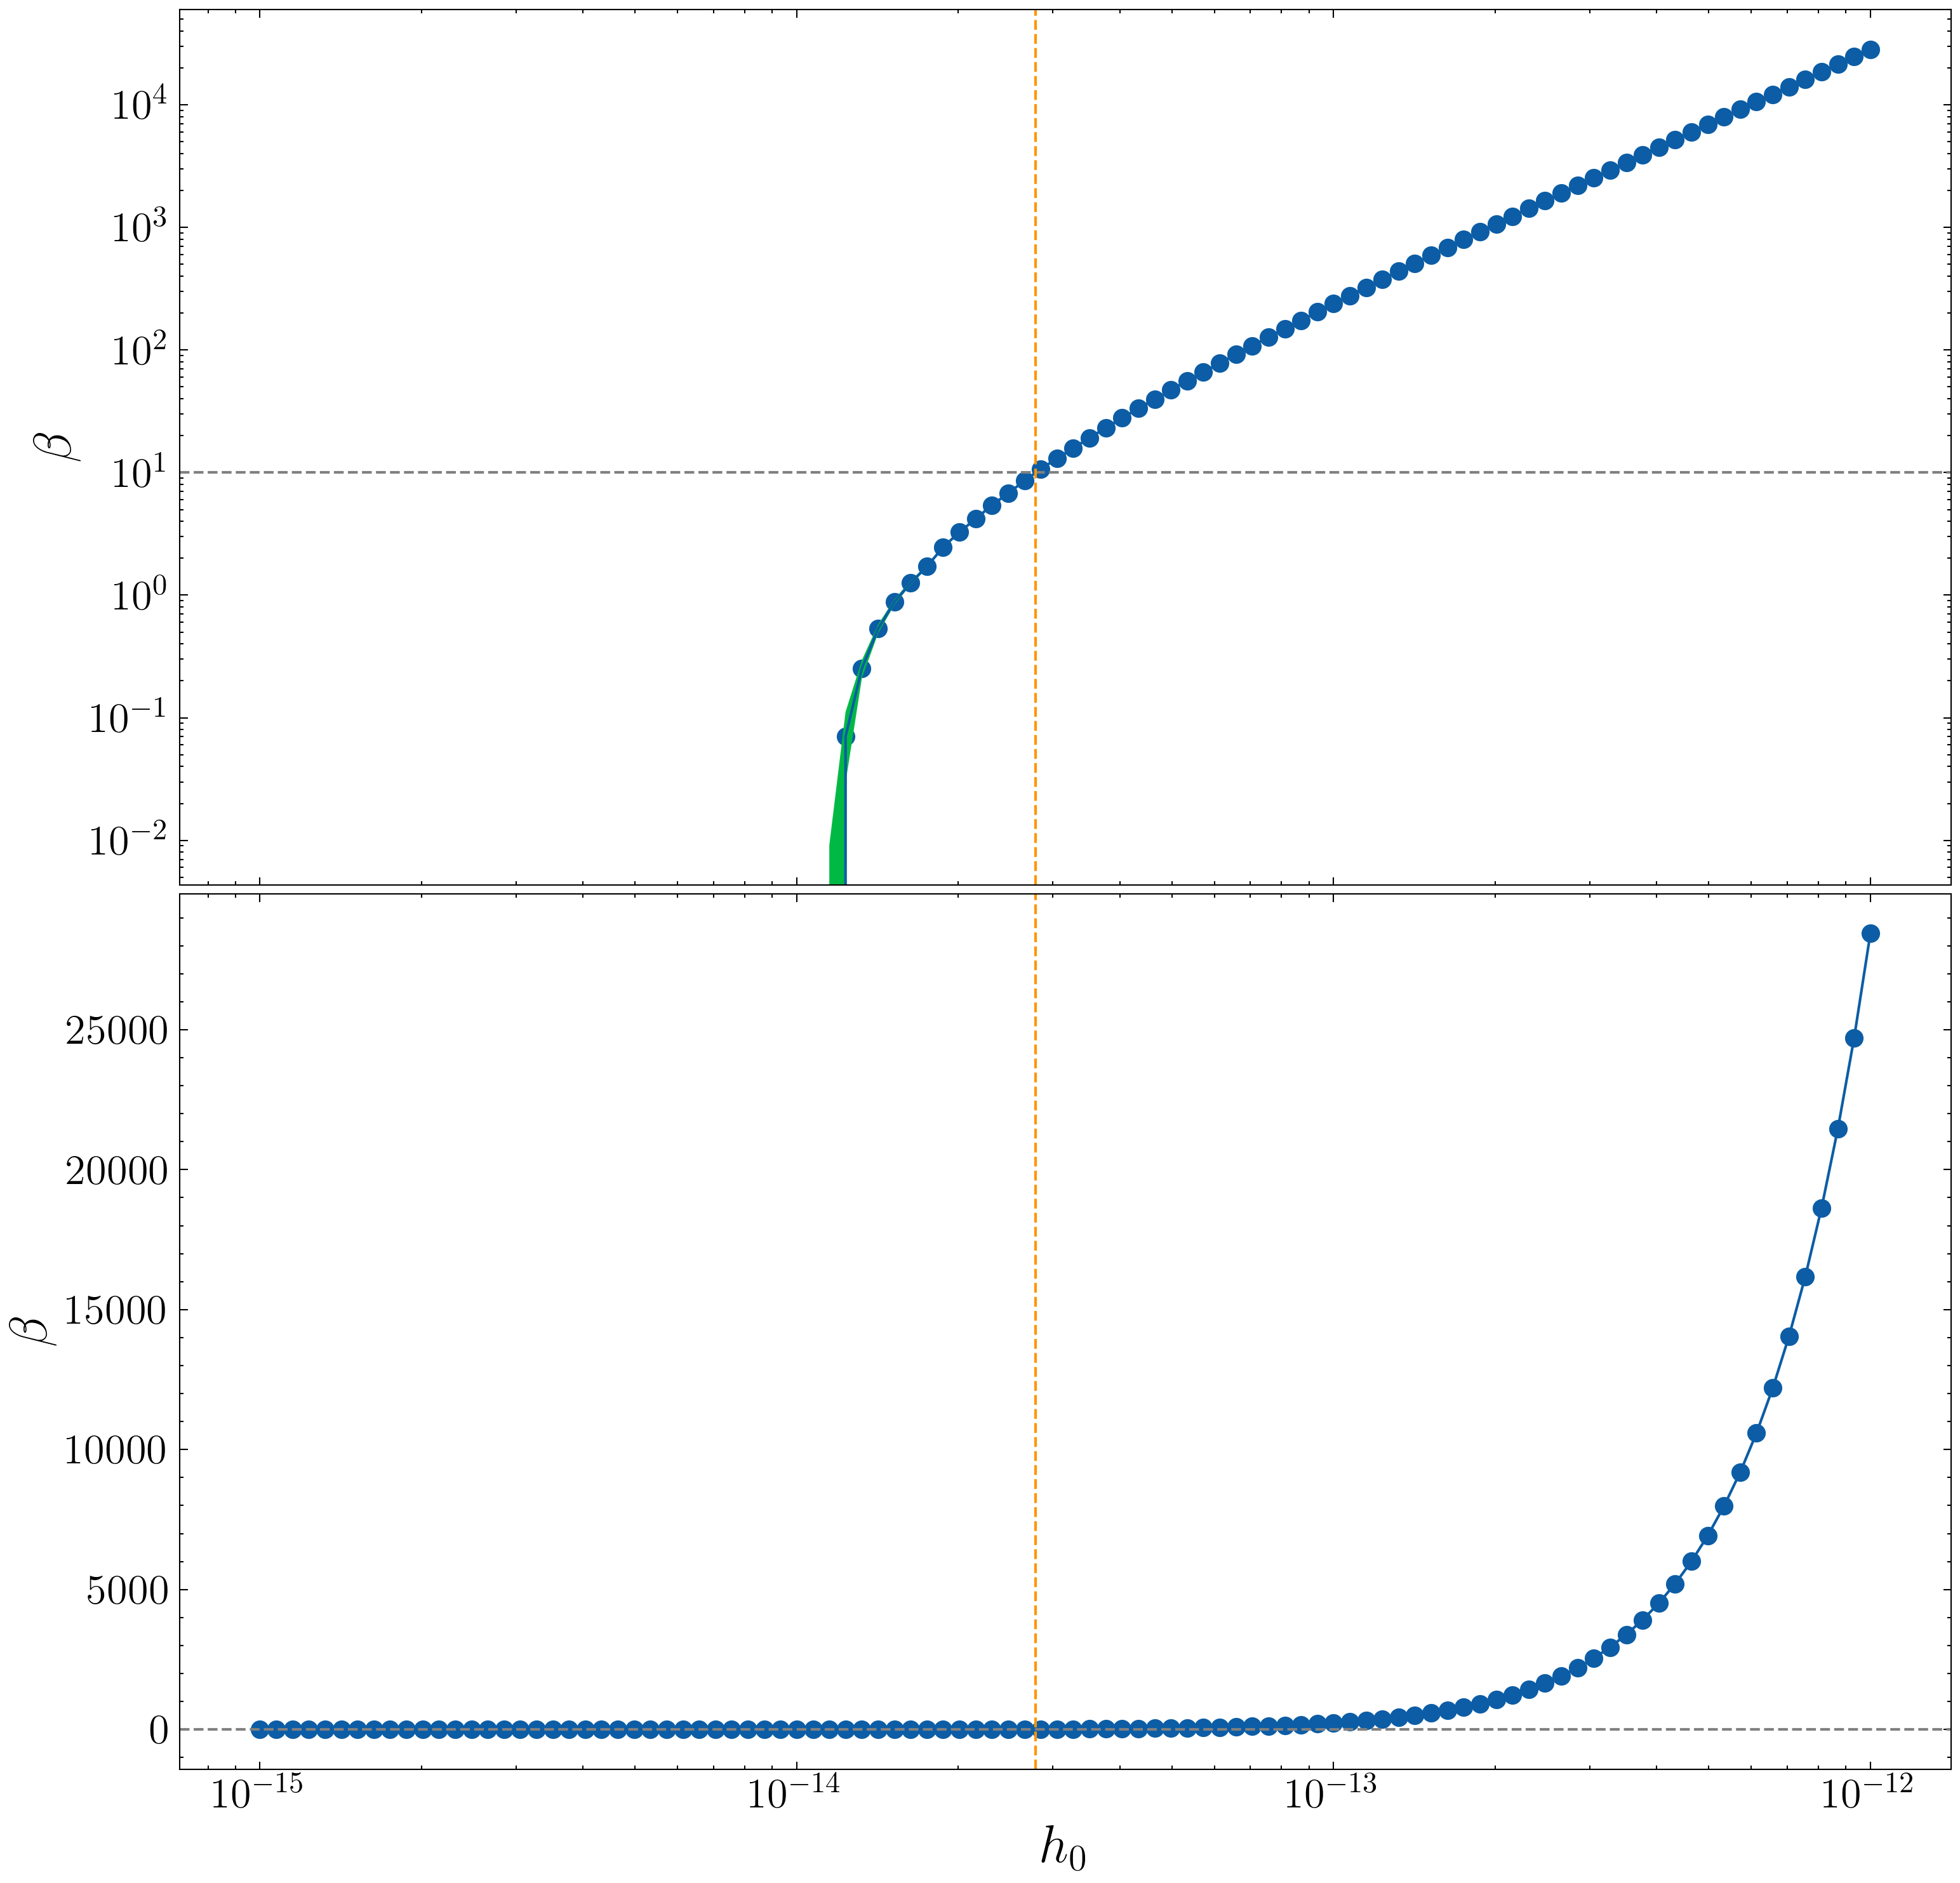
\includegraphics[width=\textwidth, height =\textwidth]{images/ExampleBayesFigure} 	
	\caption{Bayes factor (odds ratio) $\beta_{\rm M}$ between the competing models $\mathcal{M}_{\rm GW}$ a(GW present in data) and $\mathcal{M}_{\rm null}$ (GW not present in data) as a function of the signal amplitude, $h_0$, for the representative example in Table \ref{tab:parameters_and_priors}. The horizontal grey dashed line labels an arbitrary detection threshold, $\beta_{\rm M} = 10$. The minimum detectable strain for which $\beta < 10$ equals $X$. The axes are plotted on logarithmic scales. \textcolor{red}{TK:Caption TBD. Top panel is the same as bottom, just with a log y-axis. Green region is the uncertainty.}}
	\label{fig:bayes1}
\end{figure*}



\subsection{Parameter estimation}\label{sec:parameter_esimation}

In this section we...



Figure \ref{fig:corner}shows...
\begin{figure*}
	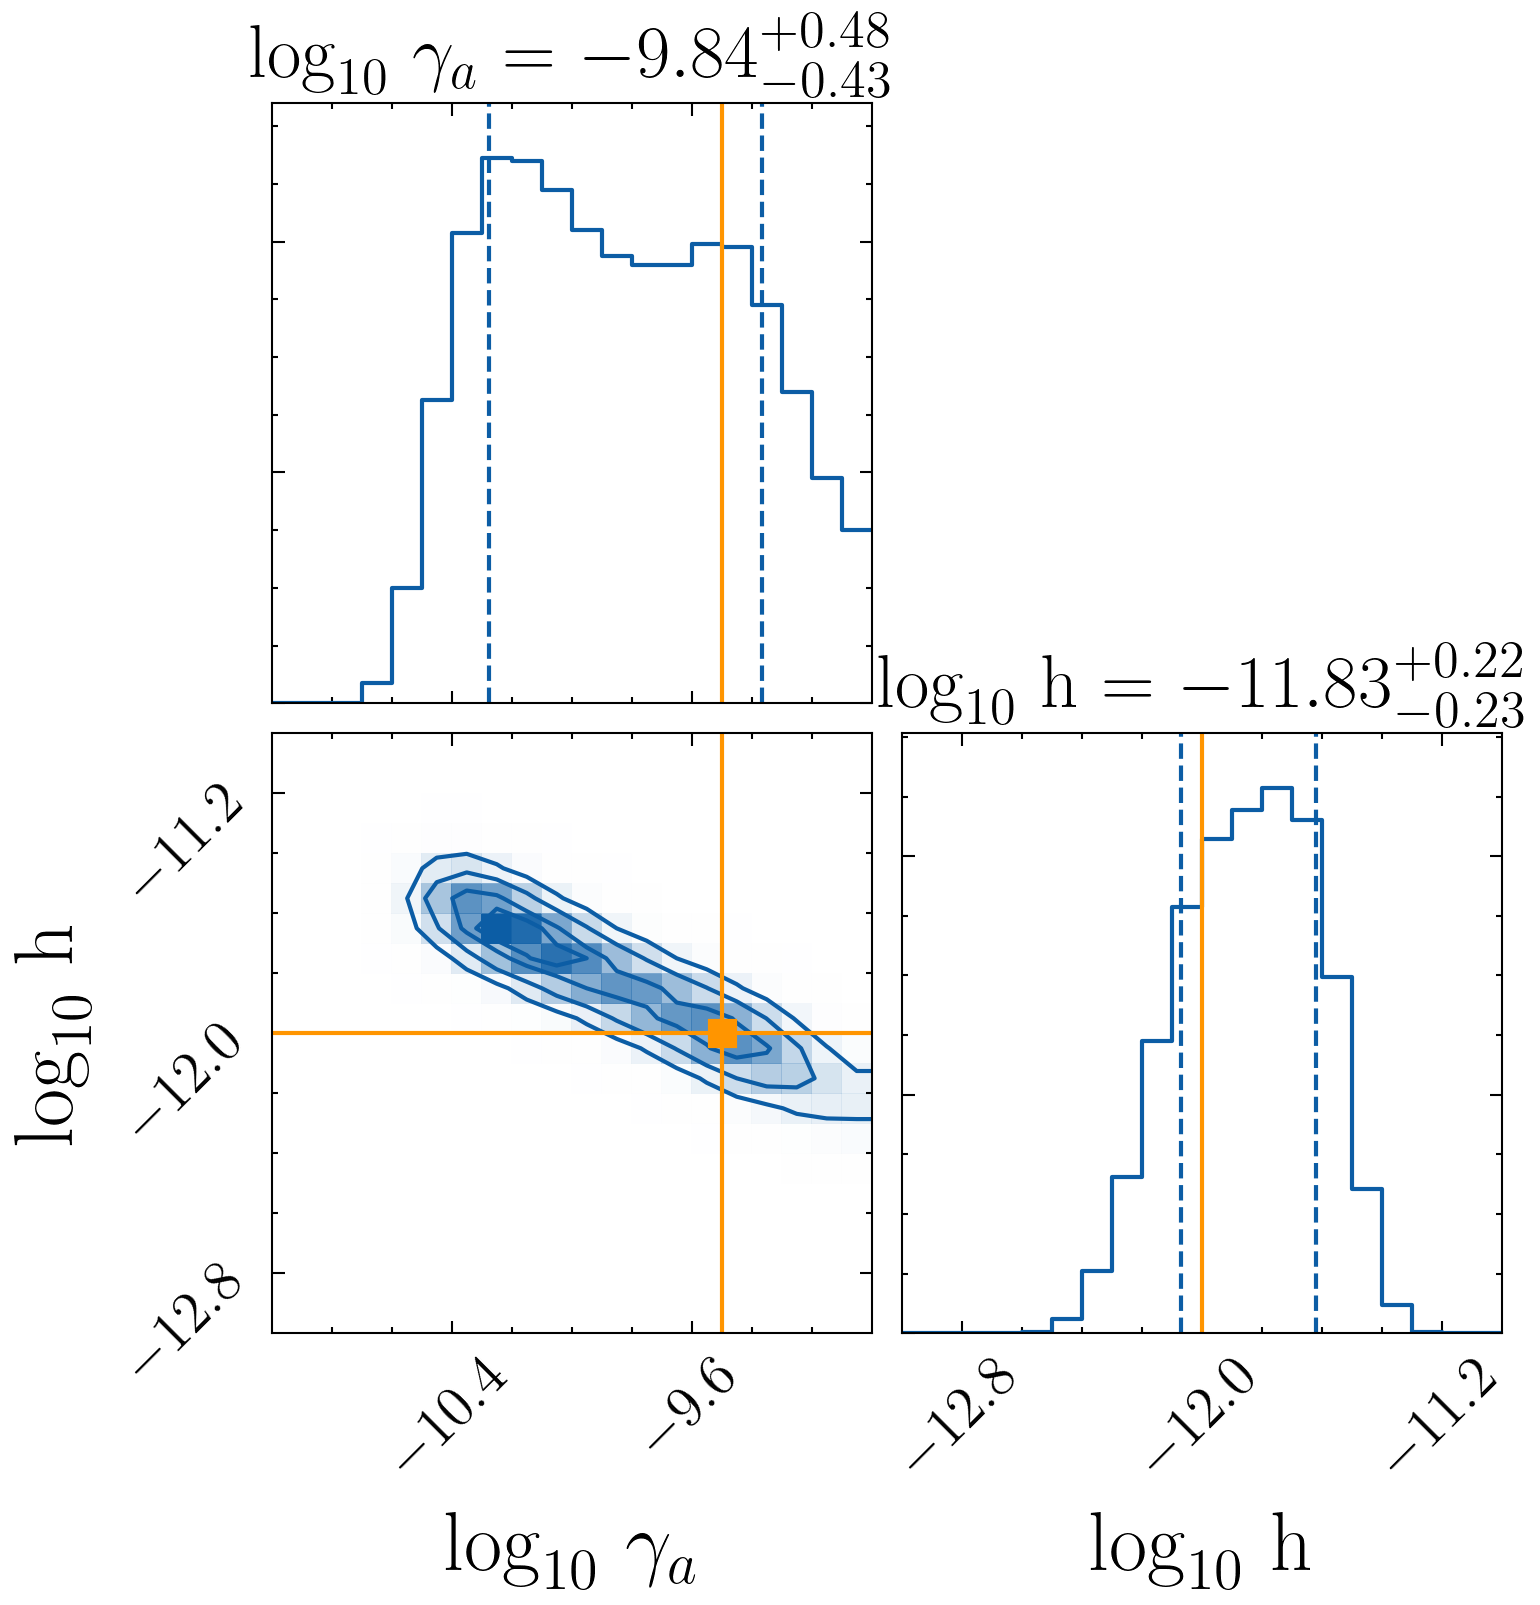
\includegraphics[width=\textwidth, height =\textwidth]{images/example_corner_plot} 	
	\caption{\textcolor{red}{TK:Caption TBD. Just GW parameters shown, but nested sampling inference is run over all $\boldsymbol{\theta}$}}
	\label{fig:corner}
\end{figure*}











\bibliographystyle{mnras}
\bibliography{example} % if your bibtex file is called example.bib



\newpage 
\appendix
\section{Derivation of the phase measurement equation}\label{appendix:measurement_equation_deriv}






















\section{Extended Kalman filter} \label{sec:kalman}
In this appendix, we describe the extended (non-linear) Kalman filter algorithm used in this paper. The Kalman filter accepts a temporal sequence of noisy measurements $\boldsymbol{Y}(t)$ as an input and recovers a temporal sequence of stochastically evolving system state variables, $\boldsymbol{X}(t)$, which are not observed directly. In this paper ${\boldsymbol{Y}}(t) = \{ f^{(n)}_{\rm m}(t_1), \dots, f^{(n)}_{\rm m}(T_{\rm obs})  \}_{1 \leq n \leq N}$ and ${\boldsymbol{X}}(t) = \{ f^{(n)}_{\rm p}(t_1), a^{n}(t_1), \dots, f^{(n)}_{\rm p}(T_{\rm obs}),a^{(n)}_{\rm p}(T_{\rm obs})   \}_{1 \leq n \leq N}$. Whilst previous state-space analyses of single continuous GW sources have used a linear Kalman filter \citep{KimpsonPTA1,KimpsonPTA2}, the non-linear relation between ${\boldsymbol{Y}}(t)$ and ${\boldsymbol{X}}(t)$ (c.f. Equation \eqref{eq:measurement}) necessitates the use of an extended (non-linear) Kalman filter \citep{zarchan2000fundamentals} in this paper. General recursion relations for the discrete-time extended Kalman filter are written down for an arbitrary dynamical system in Section \ref{sec_kalman_general}. The mapping onto the specific continuous-time state-space model in Section \ref{sec:model} is written down in Section \ref{sec_kalman_specific}.


\subsection{Recursion equations}\label{sec_kalman_general}
The extended Kalman filter operates on temporally discrete, noisy measurements $\boldsymbol{Y}_k$, which are related to a set of unobservable discrete system states $\boldsymbol{X}_k$, via a general differentiable function
\begin{equation}
	\boldsymbol{Y}_k = h \left(\boldsymbol{X}_k\right) + \boldsymbol{v}_k \ ,\label{eq:kalman1}
\end{equation}
where $h(x)$ is the measurement function or observation model, $\boldsymbol{v}_k$ is a zero-mean Gaussian measurement noise, $\mathcal{N} \sim (0,\boldsymbol{R}_k)$ with covariance $\boldsymbol{R}_k$, and the subscript $k$ labels the time-step. Similarly, the states evolve as
\begin{equation}
	\boldsymbol{X}_k = f \left(\boldsymbol{X}_{k-1}\right) + \boldsymbol{w}_{k-1} \ ,\label{eq:kalman1}
\end{equation}
where $f(x)$ is the state transition function, and $\boldsymbol{w}_k$ is a zero-mean Gaussian measurement noise, $\mathcal{N} \sim (0,\boldsymbol{Q}_k)$ with covariance $\boldsymbol{Q}_k$. \newline 


The extended Kalman filter is a recursive estimator with two distinct stages: a ``predict" stage and an ``update" stage. The predict stage predicts $\hat{\boldsymbol{X}}_{k|k-1}$, the estimate of the state at discrete step $k$, given the state estimates from step $k-1$. Specifically, the predict step proceeds as
\begin{align}
	\hat{\boldsymbol{X}}_{k|k-1} &=  f \left( \hat{\boldsymbol{X}}_{k-1|k-1}\right) \\
	\hat{\boldsymbol{P}}_{k|k-1} &=  \boldsymbol{F}_k \hat{\boldsymbol{P}}_{k-1|k-1} \boldsymbol{F}_k^\intercal + \boldsymbol{Q}_k  \ ,
\end{align}
where $\hat{\boldsymbol{P}}_{k|k-1}$ is the covariance of the prediction and $\boldsymbol{F}_k$ is the Jacobian
\begin{equation}
	\boldsymbol{F}_k = \left. \frac{\partial f}{\partial \boldsymbol{X} } \right \rvert_{	\hat{\boldsymbol{X}}_{k|k-1}} \ .
\end{equation}
The predict stage is independent of the measurements; the measurement $\boldsymbol{Y}_k$ is included to update the prediction during the update stage as follows:
\begin{align}
	\boldsymbol{\epsilon}_{k} &= \boldsymbol{Y}_k - h \left(\hat{\boldsymbol{X}}_{k|k-1} \right)\ , \\
	\boldsymbol{S}_k &= \boldsymbol{H}_k \hat{\boldsymbol{P}}_{k|k-1} \boldsymbol{H}_k^\intercal + \boldsymbol{R}_k \ , \\
	\boldsymbol{K}_k &= \hat{\boldsymbol{P}}_{k|k-1} \boldsymbol{H}_k^\intercal \boldsymbol{S}_k^{-1} \ ,\label{eq:kalman gain} \\
	\hat{\boldsymbol{X}}_{k|k} &=\hat{\boldsymbol{X}}_{k|k-1} +\boldsymbol{K}_k  \boldsymbol{\epsilon}_{k}  \ , \label{eq:kalmangainupdate} \\
	\hat{\boldsymbol{P}}_{k|k} &= \left( \boldsymbol{I} - \boldsymbol{K}_k \boldsymbol{H}_k \right) 	\hat{\boldsymbol{P}}_{k|k-1} \ .
\end{align}
where $\boldsymbol{H}_k$ is the Jacobian
\begin{equation}
	\boldsymbol{H}_k = \left. \frac{\partial h}{\partial \boldsymbol{X} } \right \rvert_{	\hat{\boldsymbol{X}}_{k|k-1}} \ .
\end{equation}
For a full review of the extended Kalman filter, including its derivation, we refer the reader to \cite{zarchan2000fundamentals}. \newline 

To apply the Kalman filter in practice means specifying the two functions $h(x)$ and $f(x)$, their associated Jacobians $\boldsymbol{H}_k$ and $\boldsymbol{F}_k$, the covariance matrices $\boldsymbol{Q}_k$ and $\boldsymbol{R}_k$, and the vectors $\boldsymbol{X}_k$
and $\boldsymbol{Y}_k$. In Section \ref{sec_kalman_specific} we describe how these components are determined for the state-space model in Section \ref{sec:state_space_formulation}. 


\subsection{State space representation of a PTA analysis}\label{sec_kalman_specific}
We apply the Kalman recursion relations in Section \ref{sec_kalman_general} to the state-space model of a PTA with $N$ pulsars described in Section \ref{sec:model} as follows. \newline 


We identify $\boldsymbol{X}(t)$ with a vector of length $N$ composed of the intrinsic pulsar frequency states, i.e. 
\begin{equation}
	\boldsymbol{X}(t) = \left(f_{\rm p}^{(1)}(t), f_{\rm p}^{(2)}(t), ..., f_{\rm p}^{(N)}(t)\right) \ .
\end{equation}
Analogously,  we package the measured pulsar frequencies as
\begin{equation}
	\boldsymbol{Y}(t) = \left(f_{\rm m}^{(1)}(t), f_{\rm m}^{(2)}(t), ..., f_{\rm m}^{(N)}(t) \right) \ .
\end{equation}
The states evolve according to the continuous stochastic differential equation (c.f. Equation \eqref{eq:frequency_evolution})
\begin{equation}
	d \boldsymbol{X} = \boldsymbol{A} \boldsymbol{X} dt + \boldsymbol{C}(t) dt + \boldsymbol{\Sigma} d \boldsymbol{B}(t) \ , \label{eq:kalmn2}
\end{equation}
where $\boldsymbol{A}$ is a diagonal $N \times N$ matrix,
\begin{equation}
	\boldsymbol{A} = \text{diag} \left(-\gamma^{(1)}, -\gamma^{(2)}, ..., -\gamma^{(N)}\right) \ ,
\end{equation}
and $\boldsymbol{C}(t)$ is a time-dependent vector with $n$-th component
\begin{equation}
	C^{(n)} =\gamma^{(n)} \left[ f^{(n)} _{\rm em} (t_1) + \dot{f}^{(n)} _{\rm em}(t_1) \, t \right] +  \dot{f}_{\rm em}(t_1)^{(n)} \ .
\end{equation}
The $N \times N$ square matrix $\boldsymbol{\Sigma}$  governs the magnitude of the increments of Brownian motion (Wiener process) $d\boldsymbol{B}(t)$, with
\begin{equation}
	\boldsymbol{\Sigma} = \text{diag} \left(\sigma^{(1)}, \sigma^{(2)}, ..., \sigma^{(N)}\right) \ .
\end{equation}

In the idealized model above, each pulsar's rotational state evolves phenomenologically according to a mean-reverting Ornstein-Uhlenbeck process, described by a Langevin equation, Equation \eqref{eq:kalmn2}, whose general solution is given by \citep{gardiner2009stochastic},
\begin{equation}
	\boldsymbol{X}(t) = e^{\boldsymbol{A} t} \boldsymbol{X}(0) + \int_0^t e^{\boldsymbol{A}(t-t')} \boldsymbol{C}(t') dt' + \int_0^t e^{\boldsymbol{A}(t-t')} \boldsymbol{\Sigma} d\boldsymbol{B}(t') \ . \label{eq:gardenier}
\end{equation} 
From Equation \eqref{eq:gardenier} we construct the discrete, recursive solution for $\boldsymbol{X}(t_k) = \boldsymbol{X}_k$ in the form of Equation \eqref{eq:kalman2}, with
\begin{align}
	\boldsymbol{F}_k &= e^{\boldsymbol{A} \Delta t } \  \\
	&= \text{diag}\left(e^{- \gamma^{(1)} \Delta t},e^{- \gamma^{(2)} \Delta t},...,e^{- \gamma^{(N)} \Delta t} \right) \ ,
\end{align}
\begin{align}
	\boldsymbol{G}_k \boldsymbol{u}_k &= \int_{t_k}^{t_{k+1}}  e^{\boldsymbol{A}\left( t_{k+1} - t' \right)}  \boldsymbol{C}(t') dt' \ , \\
	&= \left(G^{(1)}_k, G^{(2)}_k,...,G^{(N)}_k \right) ,
\end{align}
\begin{equation}
	\boldsymbol{w}_k = \int_{t_k}^{t_{k+1}} e^{\boldsymbol{A}\left( t_{k+1} - t' \right)} \boldsymbol{\Sigma} d \boldsymbol{B}(t') \ ,  \label{eq:appendix_noise}
\end{equation}
\begin{align}
	G_k^{(n)} =&    f^{(n)}_{\rm em}(t_1) + \dot{f}^{(n)}_{\rm em}(t_1)  \left(\Delta t + t_k \right) \nonumber \\ 
	&- e^{-\gamma \Delta t} \left[  f^{(n)}_{\rm em}(t_1) +\dot{f}^{(n)}_{\rm em}(t_1)  t_k \right] \ ,
\end{align}
and $\Delta t = t_{k+1} - t_k$. From Equation \eqref{eq:appendix_noise} the process noise covariance matrix is
\begin{equation}
	\boldsymbol{Q}_k \boldsymbol{\delta}_{kj}= \langle \boldsymbol{\eta}_k \boldsymbol{\eta}_j^\intercal \rangle = \text{diag} \left(Q^{(1)}, Q^{(2)},...,Q^{(N)}\right) \ ,
\end{equation}
with 
\begin{equation}
	Q^{(n)} = \frac{[\sigma^{n}]^2}{2 \gamma^{(n)}} \left[ 1 - e^{-2 \gamma^{(n)} \Delta t}\right] \ .
\end{equation}


The two remaining unspecified component matrices of the Kalman filter are the measurement matrix $\boldsymbol{H}_k$ and the measurement covariance matrix $\boldsymbol{R}_k$. These are defined straightforwardly from Equations \eqref{eq:measurement}--\eqref{eq:g_func_trig}. Specifically, 
$\boldsymbol{H}_k$ is a diagonal matrix where the $n$-th component of the diagonal is given by $g^{(n)}(t_k)$ from Equation \eqref{eq:g_func}. The measurement covariance satisfies $\boldsymbol{R}_k = E \left[ \boldsymbol{v} \boldsymbol{v}^\intercal \right] = \sigma^2_{\rm m}$ for all $k$.



%\section{References}
%\label{sec:ref_list}





%%%%%%%%%%%%%%%%Scratch space


%
%
%$f_{\rm p}^{(n)}(t)$ is related to  $f_{\rm m}^{(n)}(t)$ via a measurement equation (c.f. \eqref{eq:measurement}),
%\begin{equation}
%	f_{\rm m}^{(n)}(t) = f_{\rm p}^{(n)}\left [t-d^{(n)} \right ] g^{(n)}(t) +  \varepsilon^{(n)}(t)\ ,
%	\label{eq:measurement_appendix}
%\end{equation}
%where $d^{(n)}$ labels the distance to the $n$-th pulsar, $f_{\rm p}^{(n)}$ is evaluated at the retarded time $t-d^{(n)}$, and $\varepsilon^{(n)}(t)$ is a Gaussian measurement noise which satisfies 
%\begin{align}
%	\langle \varepsilon^{(n)}(t) \rangle &= 0 \ , \\
%	\langle \varepsilon^{(n)}(t) \varepsilon^{(n')}(t') \rangle &= \sigma_{\rm m}^2 \delta_{n,n'} \delta(t - t') \ .	\label{eq:vareps_appendix}
%\end{align}
%In Equation \eqref{eq:vareps_appendix}, $\sigma_{\rm m}^2$ is the variance of the measurement noise at the telescope and is shared between all pulsars. In Equation \eqref{eq:measurement_appendix} the measurement function $g^{(n)}(t)$ is given by \citep[e.g.][]{Maggiore}
%\begin{align}
%	g^{(n)}(t) =& 1 - \frac{ H_{ij}[q^{(n)}]^i [q^{(n)}]^j }{2 [1 + \boldsymbol{n}\cdot \boldsymbol{q}^{(n)}] } \nonumber \\
%	& \times \Big[\cos\left(-\Omega t +\Phi_0\right) \nonumber \\
%	&- \cos \left \{-\Omega t +\Phi_0 + \Omega \left[1 + \boldsymbol{n}\cdot \boldsymbol{q}^{(n)} \right]  d^{(n)} \right \} \Big ] \ ,
%	\label{eq:g_func_trig}
%\end{align}
%where $[q^{(n)}]^i$ labels the $i$-th coordinate component of the $n$-th pulsar's position vector $\boldsymbol{q}^{(n)}$, $\Omega$ is the constant angular frequency of the GW, $\boldsymbol{n}$ is a unit vector specifying the direction of propagation of the GW, $H_{ij}$ is the spatial part of the GW amplitude tensor, and $\Phi_0$ is the phase offset of the GW with respect to some reference time. \newline  



%Taking a tangible example, for pulsar J0023+0923 ATNF returns a frequency $f_{\rm em}^{(n)} (t_1) \sim 327.8$ Hz with an error $\epsilon \sim 4 \times 10^{13}$ Hz. 	The prior on $f_{\rm em}^{(n)} (t_1) \sim 327.8$ for this pulsar is then Uniform$(327.8 - 4 \times 10^{10},327.8 + 4 \times 10^{10} )$


%Alternatively, one can consider instead the alternative parametrisation in terms of $h_{+}$ and $h_{\times}$. 
%
%from Equation \ref{eq:hij} the amplitude of the plane GW perturbation at a particular sky location $\boldsymbol{n}$ is a linear combination of $h_{+}$ and $h_{\times}$. 
%
%
%
%Considering a single pulsar where the only unknown parameters of the model are $h_{+}$ and $h_{\times}$, the system is clearly under-determined - we have one equation with two unknowns - and the parameters are not identifiable 
%
%



%
%
%
%
%For instance, in Figure \ref{fig:omega_likelihood} we pass different values of $\Omega$ in the range $10^{-9}$ to $10^{-5}$ Hz into the Kalman filter, whilst holding the remaining parameters constant, and plot the retuned log-likelihood as a function of $\Omega$. 
%












%
%The second is that the log-likelihood curves for $\Omega, \delta$ and $\alpha$ are much more noisy than in the Earth-terms case. Whilst clear optima exist above the noise, and whilst local to the true value the curve becomes much more smooth, this noise presents an additional challenge to typical likelihood inference techniques which perform best on smooth likelihoods with a single clear global optima. It affects these parameters in particular since Equation \eqref{eq:g_func_trig} contains a phase term $\Omega \left(1 + \boldsymbol{n}\cdot \boldsymbol{q}^{(n)} \right)  d^{(n)}$, which is essentially a combination of these 3 parameters ($ \boldsymbol{n}$ is defined by $\delta$ and $\alpha$). When calculating a likelihood we are asking "How likely is this data, given these parameters". The inclusion of the pulsar terms results in effectively 2 continuous waves with different frequencies and phase. Perturbing e.g. $\alpha$ influences wave 1 in some non-liner way and wave 2 in some different non linear way. Whether this new set of parameters makes the data more likely depends on the particular combination of those two waves. \textcolor{red}{TK: this explanation of why these parameters is clunky because it is not properly clear to myself. Think in terms of $g(\theta)$ and $g(\hat{\theta})$}. 






%
%. In turn, each posterior distribution has a median value. We plot the distribution of these medians over the 1000 noise realisations for each parameter of $\boldsymbol{\theta}_{\rm gw}$ in Figure \ref{fig:median_distriubutins}. For each of these distributions we can also calculate the median value (i.e. the median of the medians) and compare it with the true injection value. This is shown by the red and orange dashed lines respectively in the Figure. Analogous to the results we saw in Figure \ref{fig:corner_plot_2}, the distributions of the median values of the parameters $\Omega, \Phi_0, \psi, \delta$ and $\alpha$ are very narrow, with a generally small discrepancy between the inferred value and the injected value. Conversely, the distributions for $\iota$ and $h_0$ are much broader and exhibit a bias of $\sim 0.18$ radians and $0.17 \times 10^{-12}$ respectively. This agrees with the results we discussed for the 9 noise realisations in Figure \ref{fig:corner_plot_2} where a bias in $\iota$ and $h_0$ was also observed. In addition to  $\iota$ and $h_0$  exhibiting a strong bias, the parameters $\psi$ and $\alpha$ also exhibit a small bias of magnitude $\sim 0.1$ and $\sim 0.04$ radians respectively. This bias is again a result of dropping the pulsar terms from the measurement equation and will be discussed in . 












%%%%%%%%%%%%%%%%%%%%%%%%%%%%%%%%%%%%%%%%%%%%%%%%%%


% Don't change these lines
\bsp	% typesetting comment
\label{lastpage}
\end{document}

% End of mnras_guide.tex
